\documentclass[hyperref=colorlinks]{beamer}
\mode<presentation>
\usetheme{iclpt}
\setbeamertemplate{navigation symbols}{}
\setbeamertemplate{headline}{
\begin{beamercolorbox}[leftskip=.2cm,rightskip=.2cm,topskip=.2cm,ht=1.1cm,dp=0.1cm,wd=\textwidth]{institute in head/foot}
  
\includegraphics[height=1cm]{icl.pdf}
  \hfill
  
\includegraphics[height=1cm]{../Pics/CMS-Color.pdf}
\end{beamercolorbox}
}
\setbeamertemplate{footline}{
\begin{beamercolorbox}[ht=.55cm,dp=0.4cm,wd=\textwidth,leftskip=.3cm]{author in head/foot}%
  \begin{minipage}[c]{5cm}%
    \usebeamerfont{author in head/foot}
    \insertshortauthor 
    \insertshorttitle
    \end{minipage}\hfill%
  \insertframenumber{} / \pageref{lastframe}
  \hfill
  \begin{minipage}{6cm}
    \hfill
  \end{minipage}
\end{beamercolorbox}%
}

\usepackage{color}
\usepackage{tabularx,colortbl}
\usepackage{graphicx}
\usepackage{pdfpages}
\usepackage{feynmp}
\usepackage{tikz}
\usetikzlibrary{calc, shapes, backgrounds,arrows,positioning}
\DeclareGraphicsRule{*}{mps}{*}{}

\title{\vspace{-0.2cm} Dimuon bump cross check}
\subtitle{\vspace{-0.7cm}}
\author[]{}%\underline{P. Dunne}} % A.M. Magnan and A. Nikitenko Joao Pela with \\ R. Aggleton, J. Brooke: Bristol \\ C.Asawangtrakuldee, Q.Li: Peking \\ P. Srimanobhas: Chulalongkorn \\ S. Kumar, K. Mazumdar: Mumbai}
\titlegraphic{
  \vspace{-0.7cm}
  %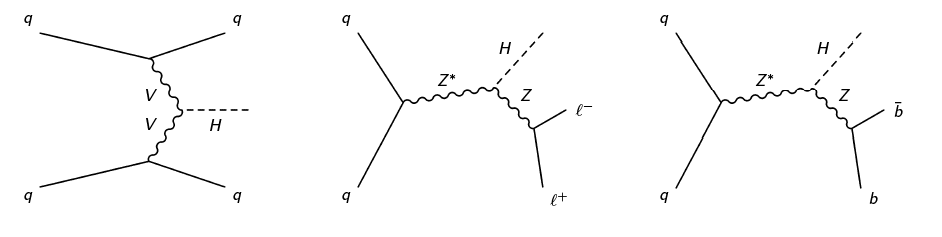
\includegraphics[width=\textwidth]{TalkPics/invcomb021213/feyndiags}
  %% \begin{fmfgraph*}(100,70)
  %%         \fmfleft{i1,i2}
  %%         \fmfright{o1,o2,o3}
  %%         \fmf{fermion}{i1,v1,o1}
  %%         \fmf{fermion}{i2,v2,o3}
  %%         \fmf{phantom,tension=4/5}{v1,v2}
  %%         \fmffreeze
  %%         \fmf{photon,label=$W,,Z$}{v1,v3}
  %%         \fmf{photon,label=$W,,Z$}{v2,v3}
  %%         \fmf{dashes}{v3,o2}
  %%         \fmflabel{$q$}{i1}
  %%         \fmflabel{$q$}{i2}
  %%         \fmflabel{$q$}{o1}
  %%         \fmflabel{$q$}{o3}
  %%         \fmflabel{$H$}{o2}
  %%       \end{fmfgraph*}
}
\date{}
\begin{document}
\begin{fmffile}{higgsexoupdatefeyndiags}
\tikzstyle{every picture}+=[remember picture]

%TITLE PAGE
\section{Title}
\begin{frame}
  \titlepage
  
\end{frame}

\begin{frame}
  \frametitle{Reminder}
  \begin{block}{}
    \begin{itemize}
    \item Sasha showed a 5-6 sigma bump in the dimuon mass distribution last week
    \item Much effort is being put into cross-checking it in the higgs-exo group
    \item We have the full single mu primary dataset processed for our trigger efficiency studies
    \end{itemize}
    \end{block}
\end{frame}

\begin{frame}
  \frametitle{Ntuples}
  \begin{block}{}
    \begin{itemize}
    \item Use common ntuple format of $H\rightarrow\tau\tau/inv.$
    \item Ntuples have no skimming so all events present
    \item Make Light trees requiring events pass data quality cuts and have two muons with $M_{\mu\mu}<70$ GeV and a CSVL b jet
    \item All my plots are of dimuon mass in GeV
    \end{itemize}
  \end{block}
\end{frame}

\begin{frame}
  \begin{block}{}
    \begin{itemize}
    \item Require: 2 $\mu$ with $p_{T}>25$ GeV + jet 1 central and with CSV$>$0.783
    \item Right hand plot also has extra jet veto
    \item Both show 2-3 sigma bump
    \end{itemize}
  \end{block}
  \centering
  \begin{columns}
    \column{.5\textwidth}
    My Plot
    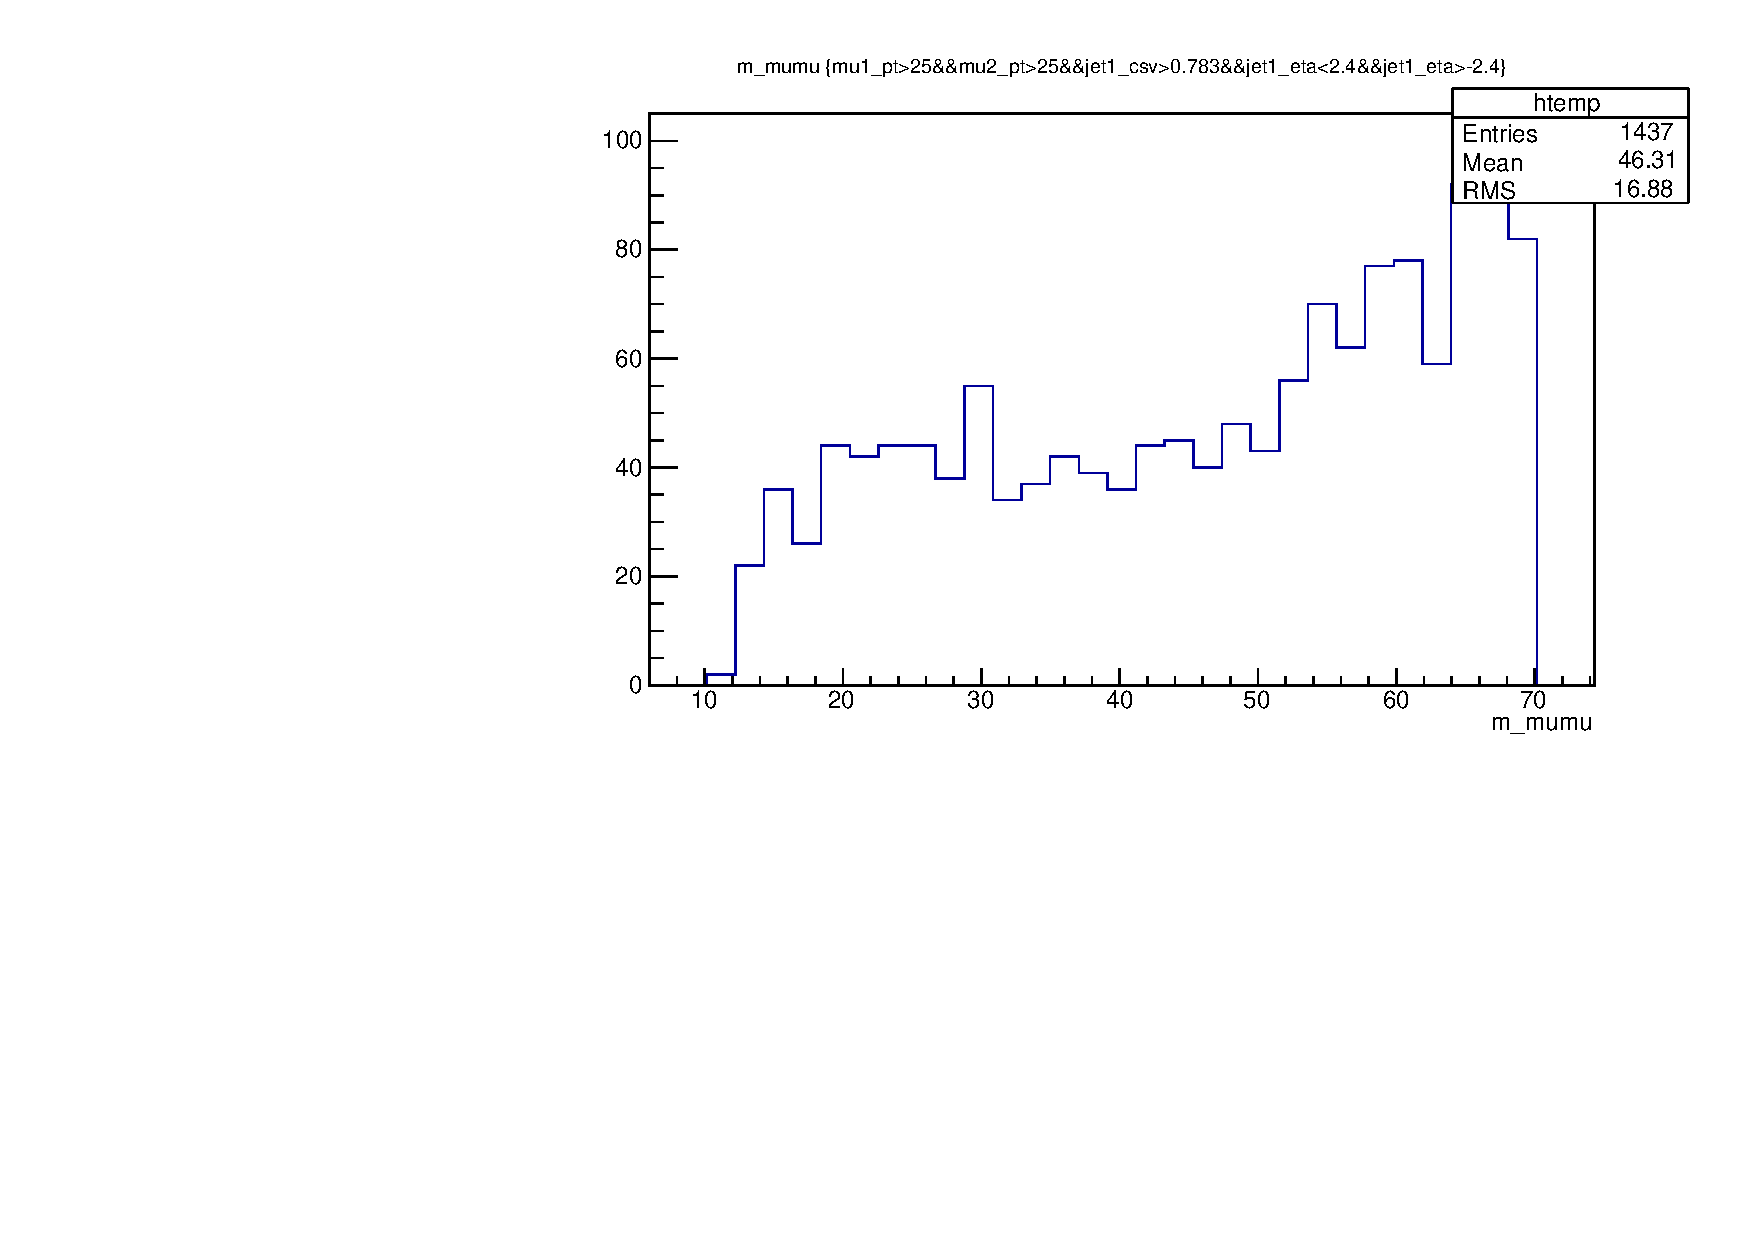
\includegraphics[width=1.1\textwidth]{TalkPics/sashacheck140715/mmumu_firstlook.pdf}
    \column{.5\textwidth}
    September 1st 2014 plot
    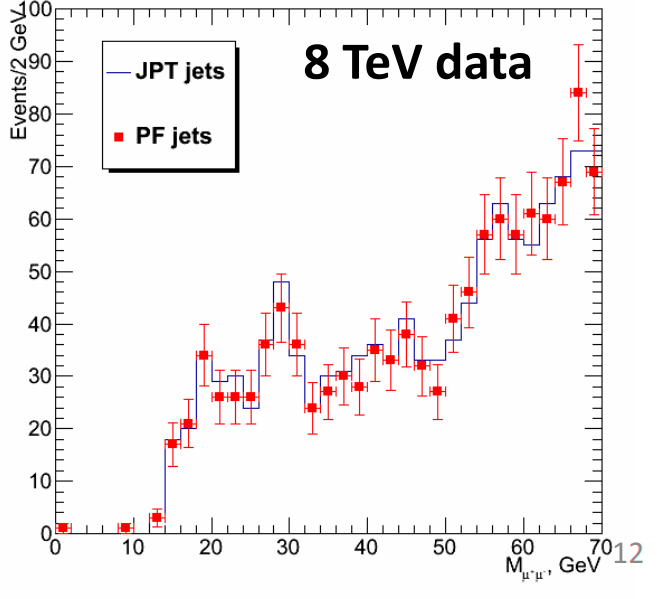
\includegraphics[width=.9\textwidth]{TalkPics/sashacheck140715/dimuonoriginal.png}
  \end{columns}
  
\end{frame}

\begin{frame}
  \frametitle{Same binning}
  \begin{block}{}
    \begin{itemize}
    \item Previous slide binning was slightly different to September 1st
    \item Change to same 2 GeV bins:
    \item[-] Left bins starting at 0, right starting at 1
    \item Significance very sensitive to minor details
    \end{itemize}
  \end{block}
  \centering
  \begin{columns}
    \column{.5\textwidth}
    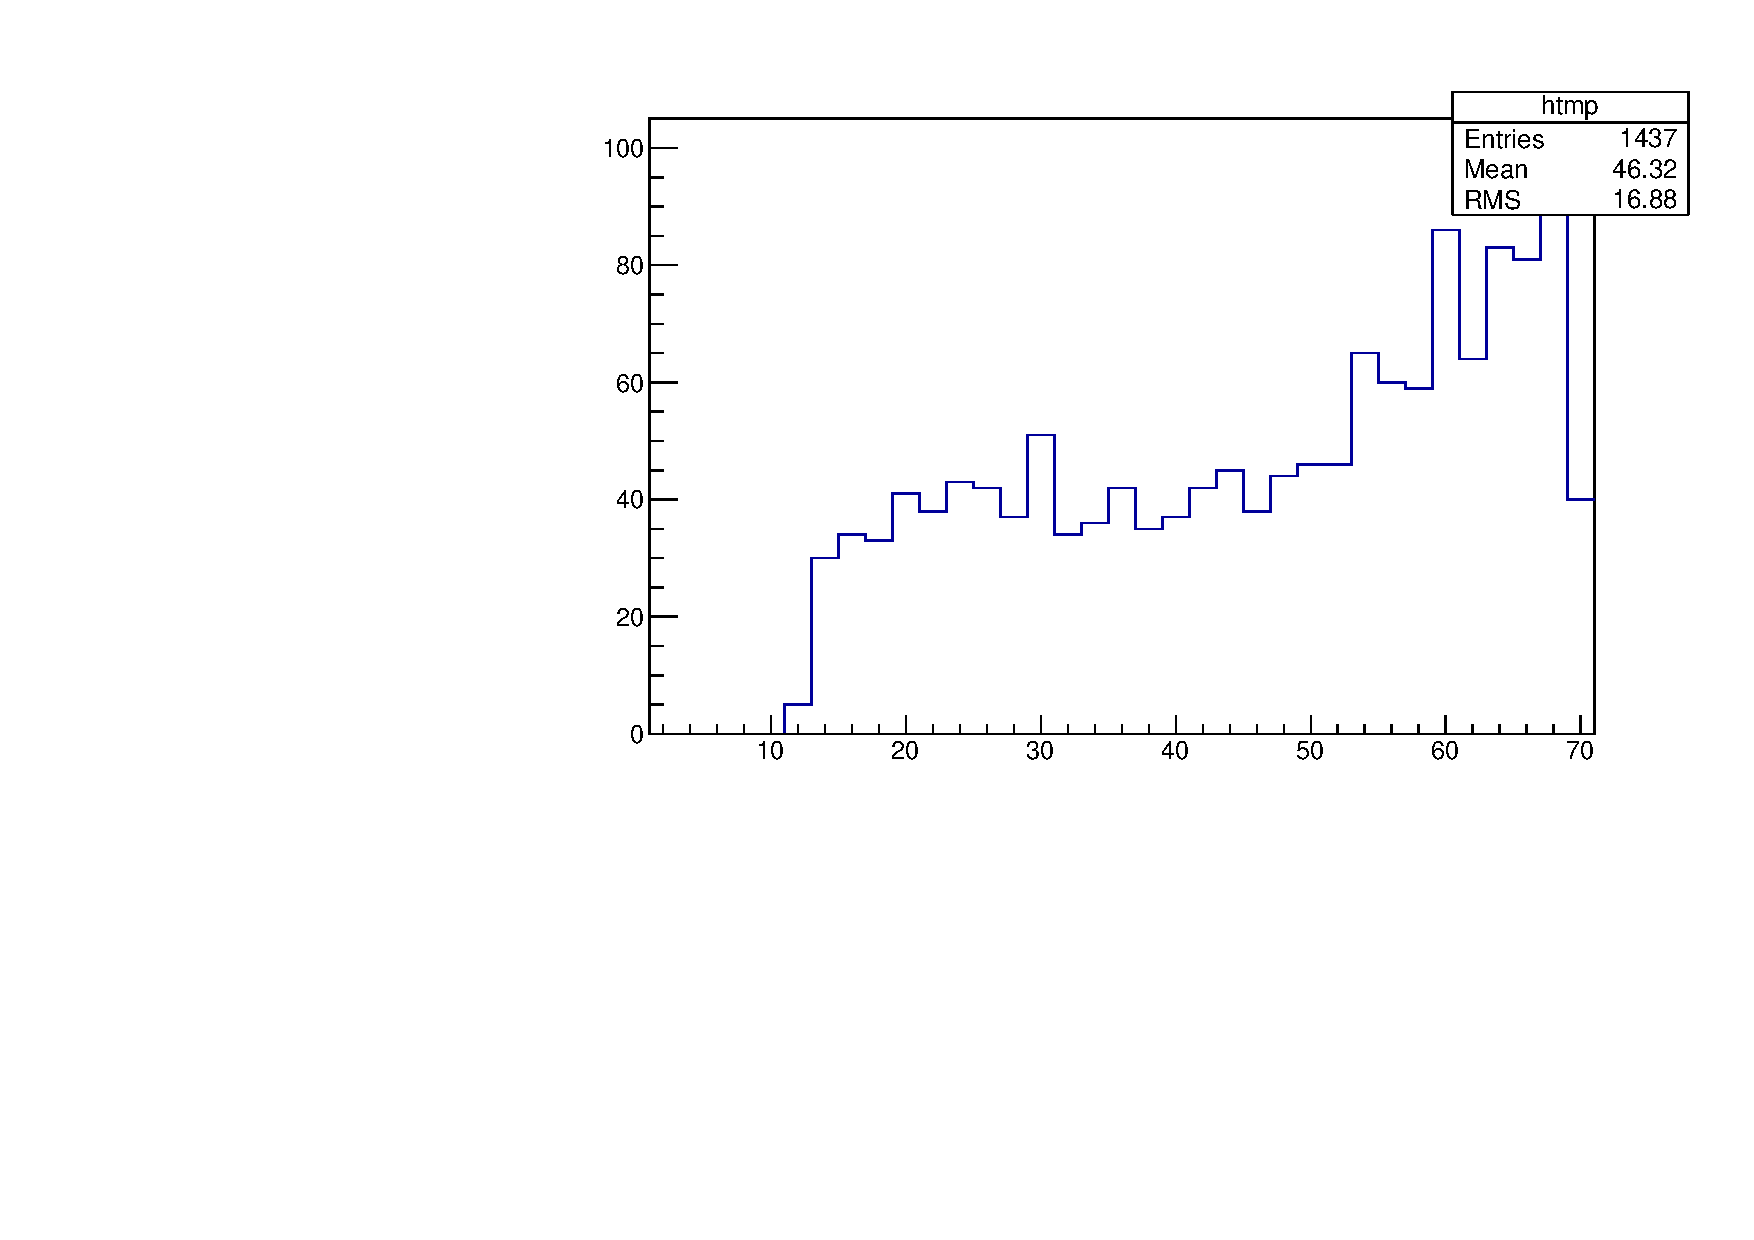
\includegraphics[width=1.1\textwidth]{TalkPics/sashacheck140715/mmumuoddbins.pdf}
    \column{.5\textwidth}
    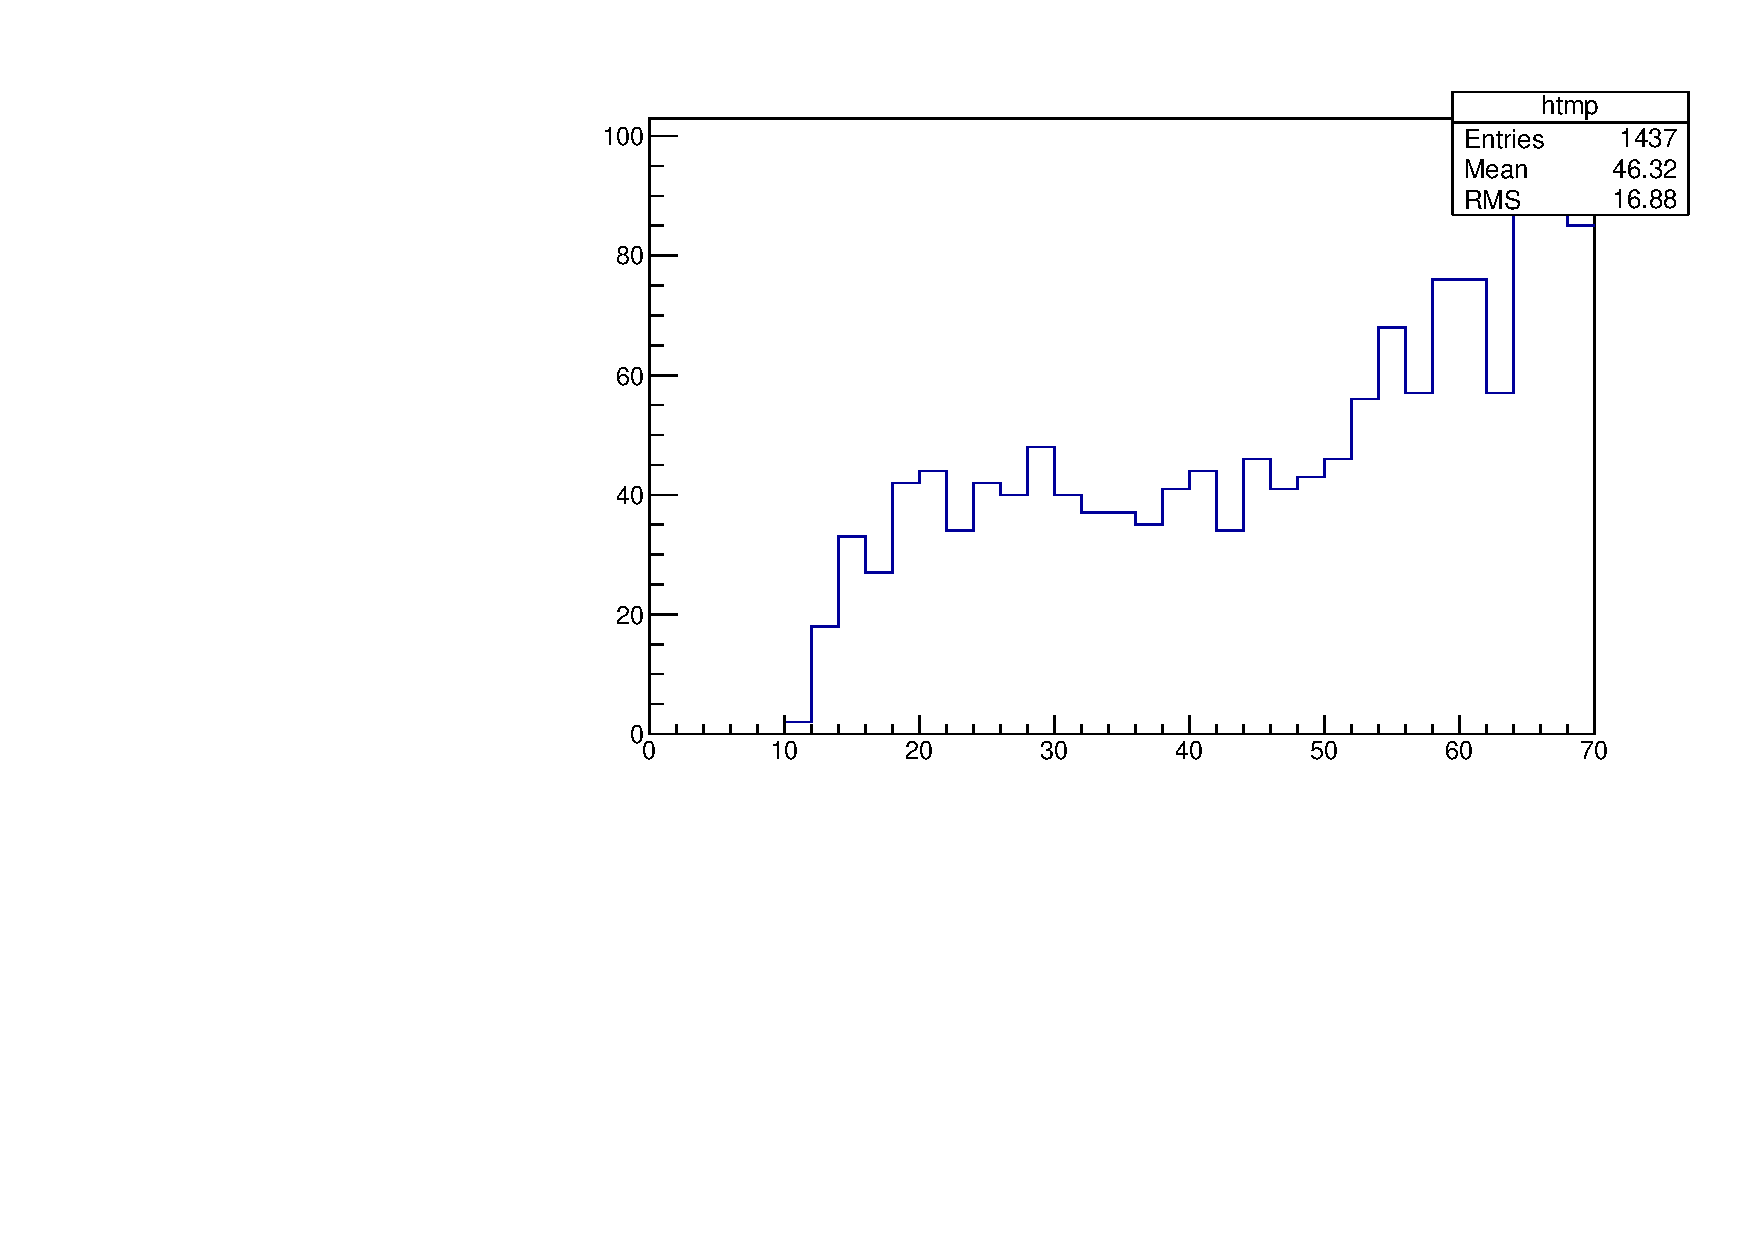
\includegraphics[width=1.1\textwidth]{TalkPics/sashacheck140715/mmumuevenbins.pdf}
  \end{columns}
\end{frame}

\begin{frame}
  \frametitle{Adding cuts - additional central jet veto}
  \begin{block}{}
    \begin{itemize}
    \item Start adding the other cuts present in Sasha et al analysis
    \item[-] First go from requiring jet 1 central and with CSV$>0.783$ to requiring that there is one and only one central jet and it has CSV$>$0.783
    \end{itemize}
  \end{block}

    \centering
    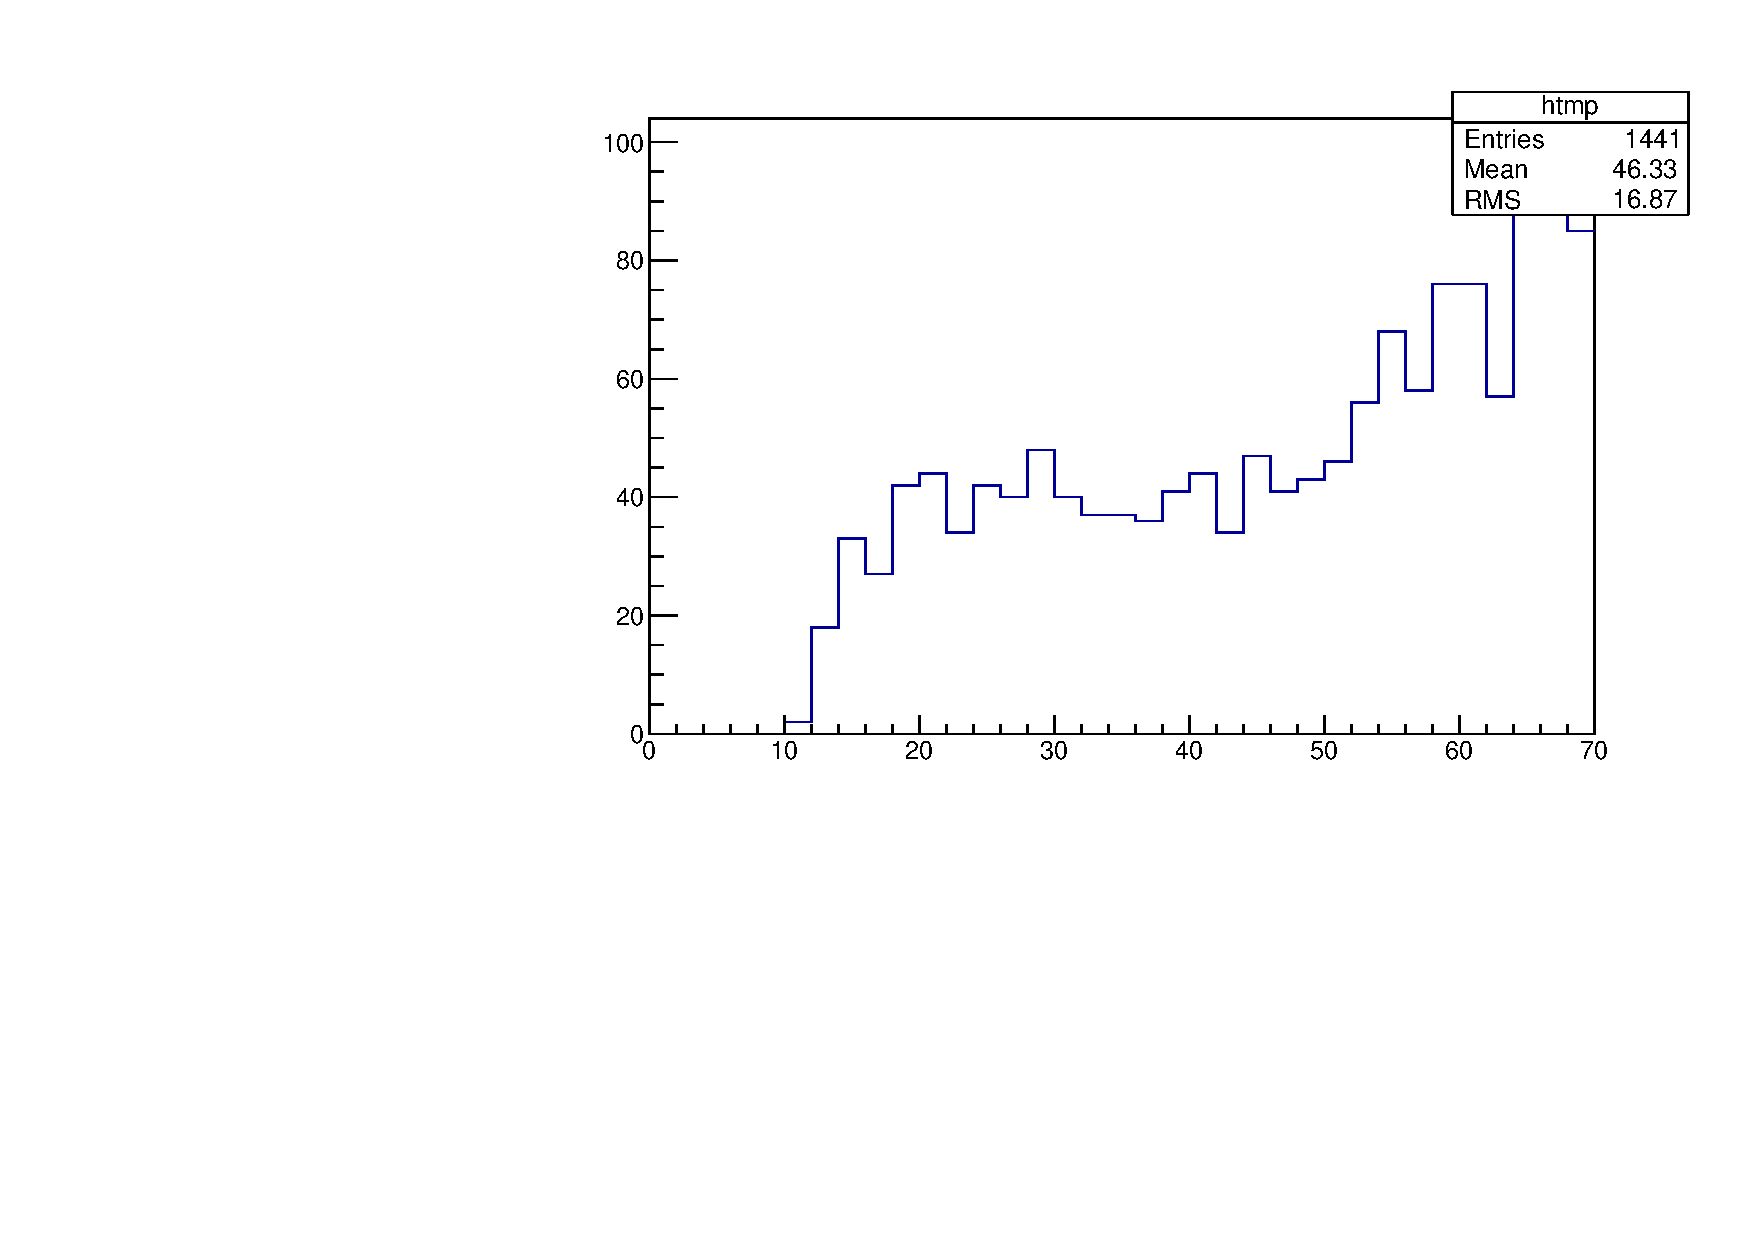
\includegraphics[width=.5\textwidth]{TalkPics/sashacheck140715/mmumu_onecentralbjet.pdf}
\end{frame}

\begin{frame}
  \frametitle{Adding cuts - b tag threshold}
  \begin{block}{}
    \begin{itemize}
    \item Next noticed that 0.783 is medium WP for CSVV1 not CSV
    \item[-] Change threshold to CSVM threshold=0.679
    \end{itemize}
  \end{block}

    \centering
    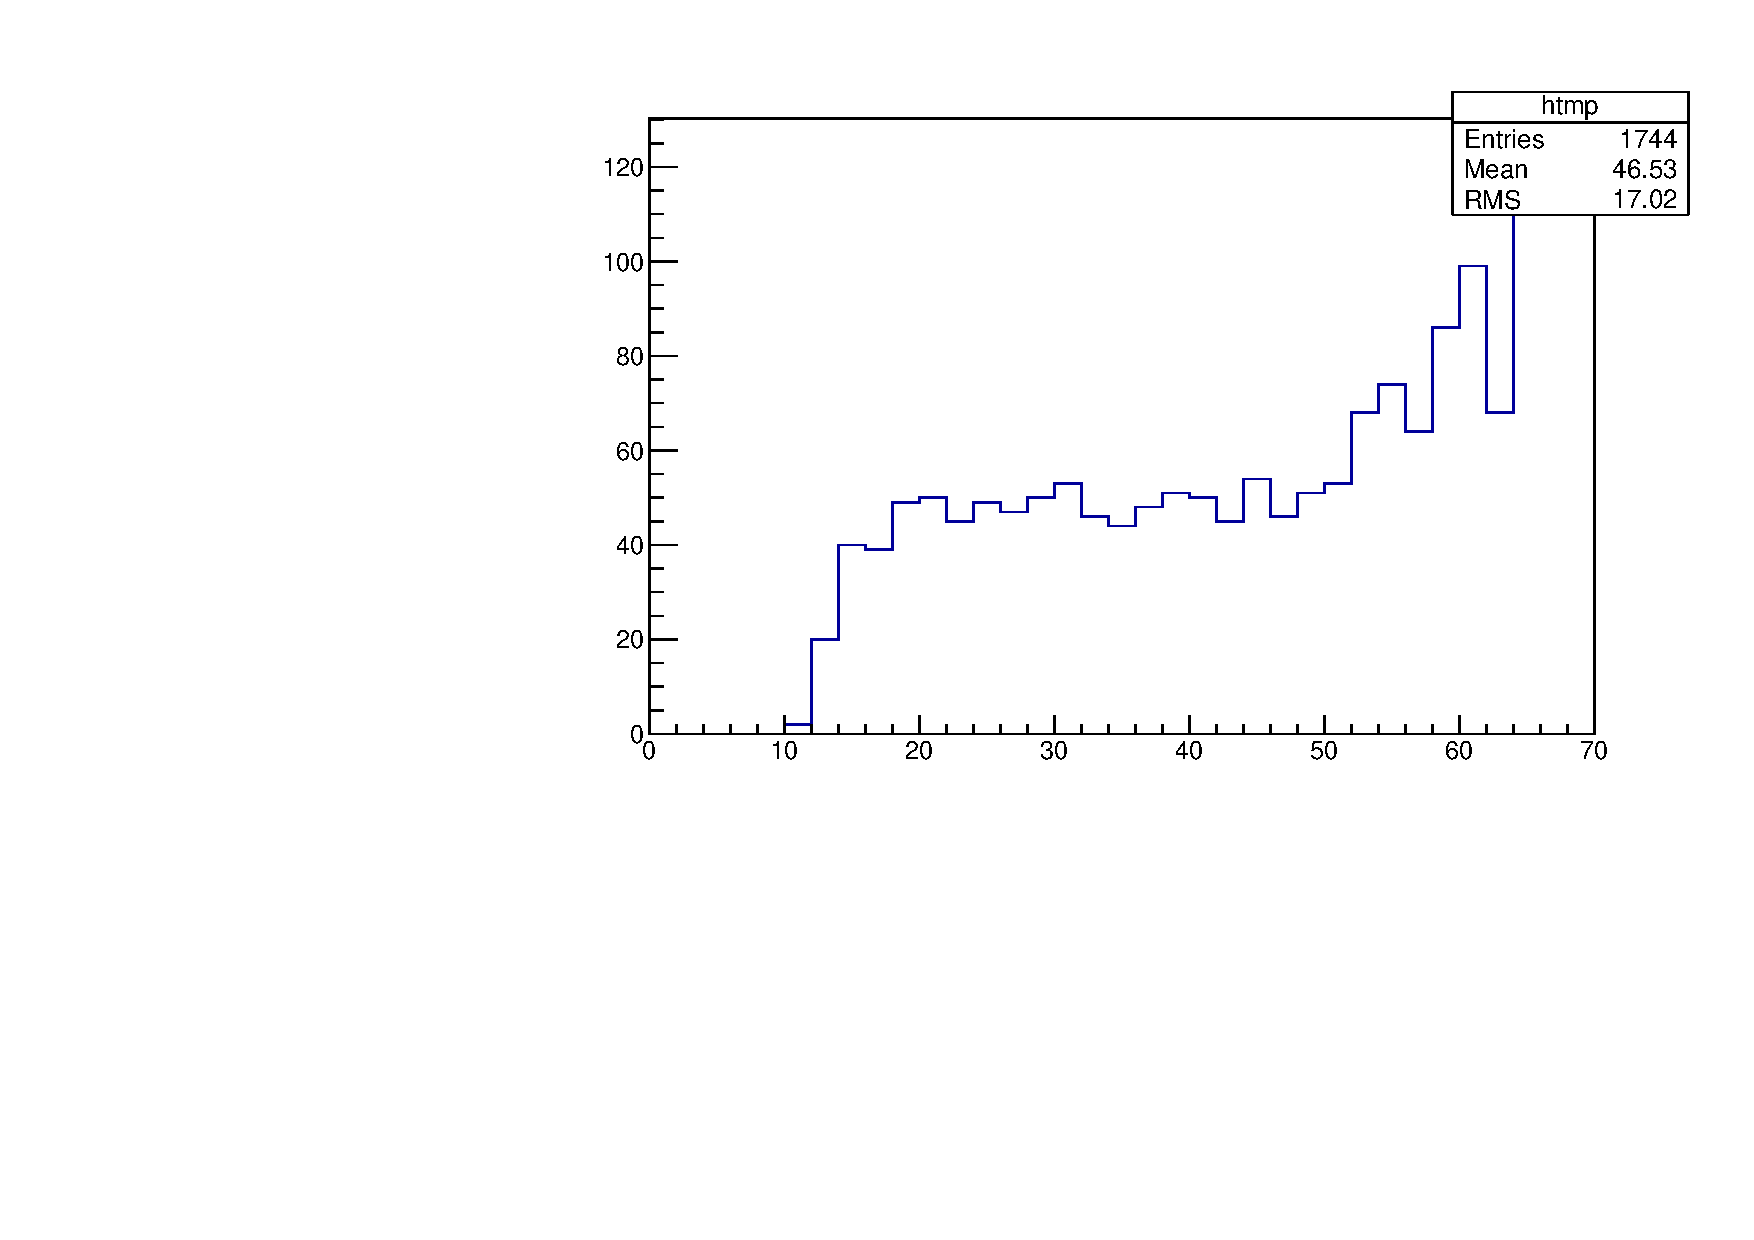
\includegraphics[width=.5\textwidth]{TalkPics/sashacheck140715/mmumu_onecentralcsvmbjet.pdf}
\end{frame}

\begin{frame}
  \frametitle{Adding cuts - forward jet}
  \begin{block}{}
    \begin{itemize}
    \item Add requirement of at least one forward jet $p_{T}>30$ GeV
    \item Almost all events removed
    \item Could point to forward jet ID difference
    \end{itemize}
  \end{block}

    \centering
    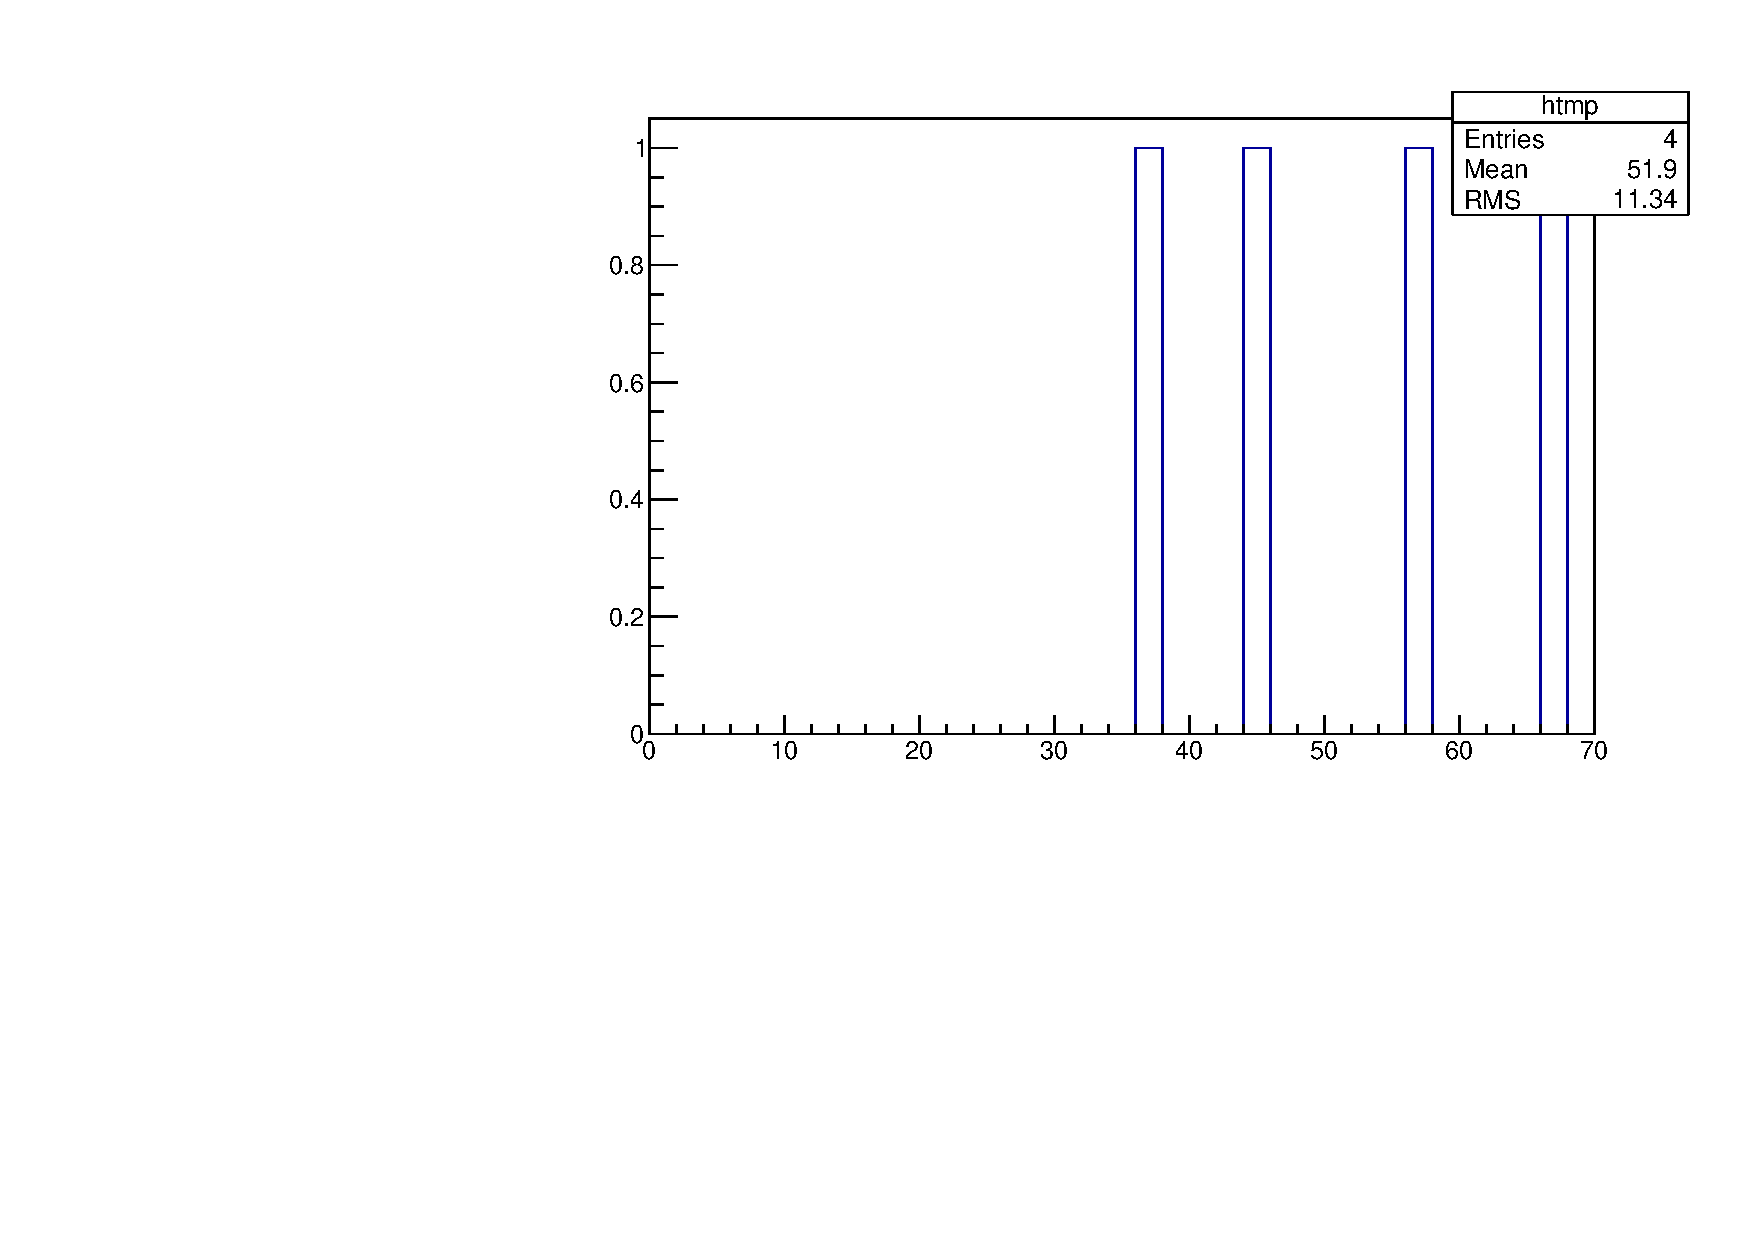
\includegraphics[width=.5\textwidth]{TalkPics/sashacheck140715/mmumu_forwardjet.pdf}
\end{frame}


\begin{frame}
  \label{lastframe}
  \begin{block}{Caveats}
    \begin{itemize}
    \item All prepared very quickly
    \item Small number of files had xrootd issue when reading
    \item[-] Shouldn't cause big effect unless all of bump is in a few runs coincidentally missed
    \end{itemize}
  \end{block}
  \begin{block}{Summary}
    \begin{itemize}
    \item $\sim$3 sigma bump seen last year appears to be present in my ntuples too
    \item Moving cuts towards Sasha et als appears to reduce the bump
    \item Further investigation with Sasha needed
    \end{itemize}
  \end{block}
\end{frame}

\begin{frame}
  \frametitle{Backup}
\end{frame}

\end{fmffile}
\end{document}
